\chapter{船岸连接系统关键技术问题与分析}

\section{船用岸电电源系统结构}

综合对比目前各种己知的低压岸电变流系统拓扑结构,采用三相PWM整流和三相PWM逆变双全控系统是最理想的选择,
也最符合岸电电源系统的实际需求其拓扑结构图如图\ref{fig:岸电电源变流系统}所示。

\begin{figure}[!htp]
	\centering
	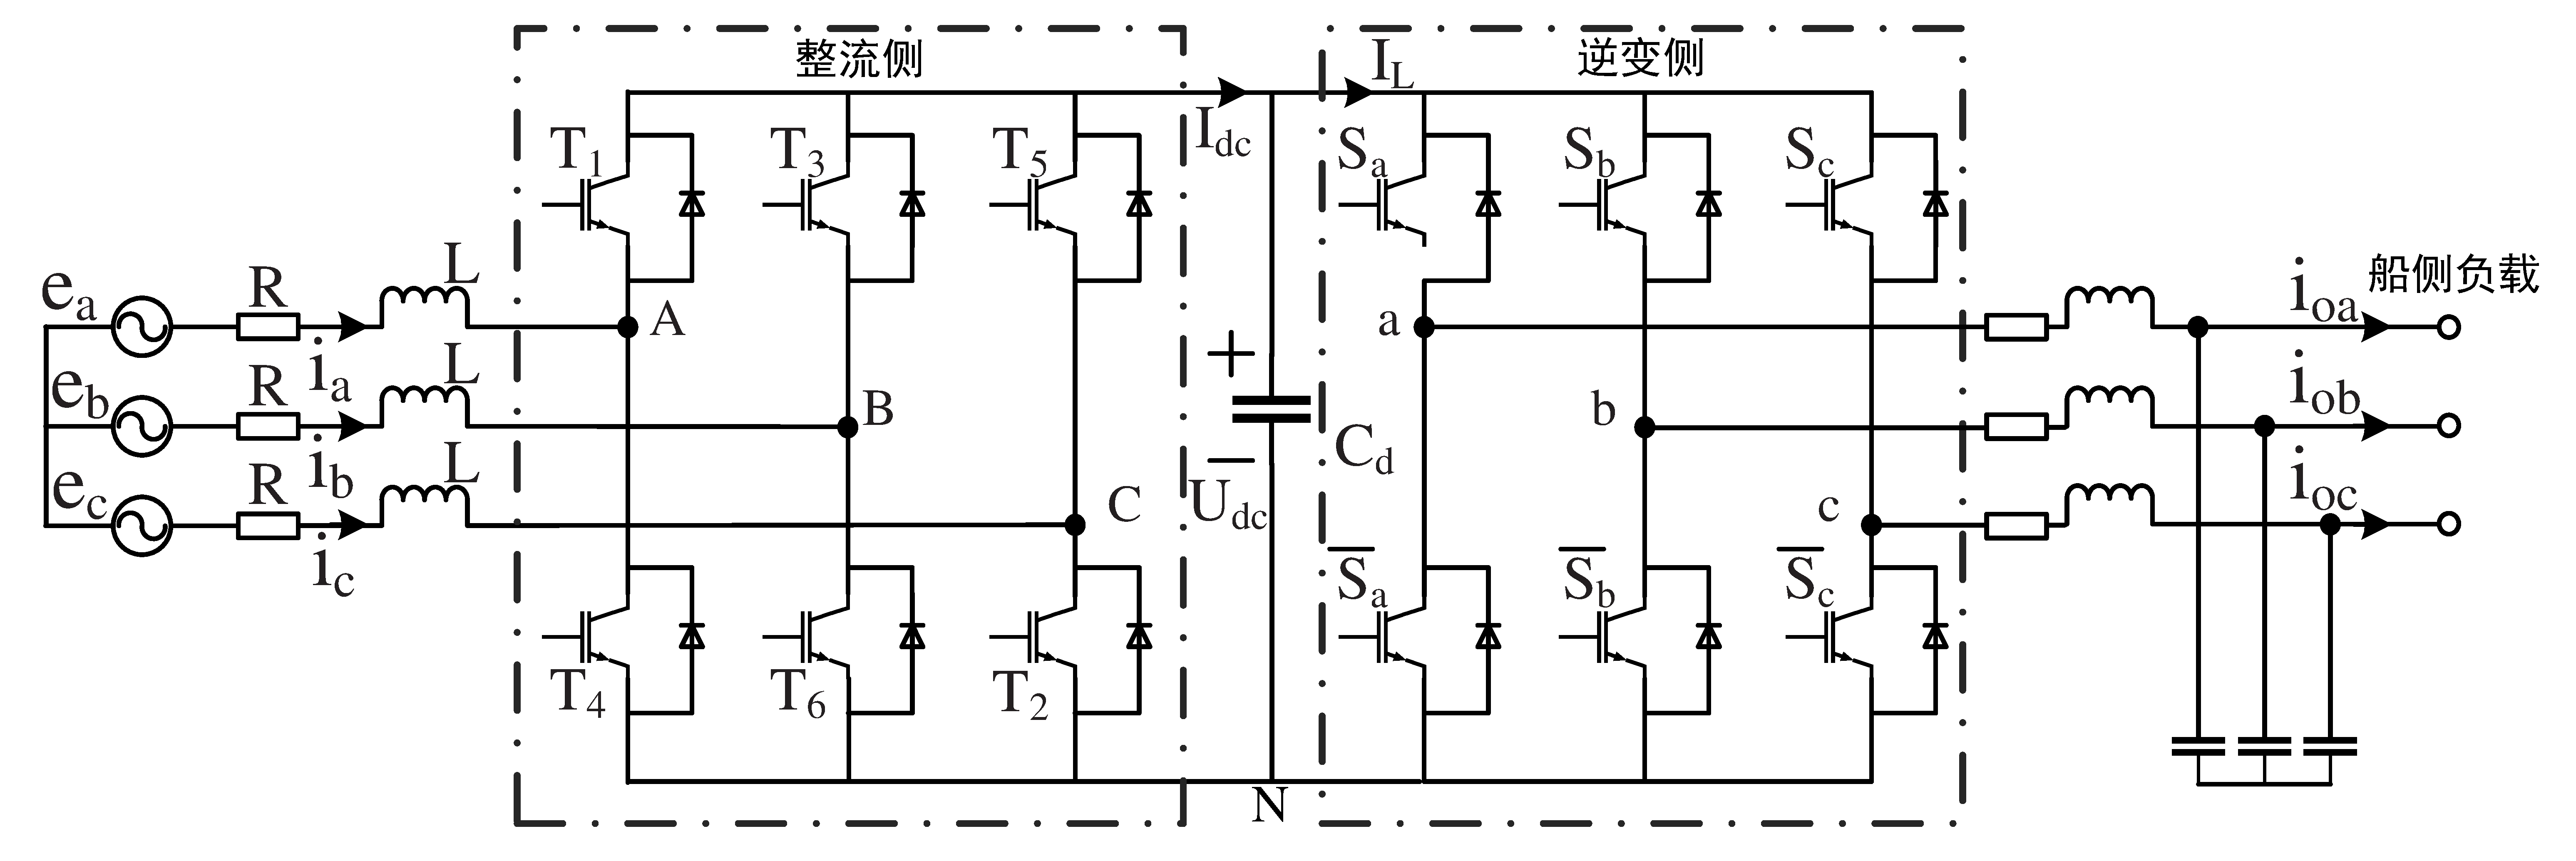
\includegraphics[width=\textwidth]{chapter3/变流器拓扑.pdf}
	\caption{岸电电源变流系统}
	\label{fig:岸电电源变流系统}
\end{figure}

\section{岸侧变流器系统模型与分析}

\subsection{变流器整流侧模型}

\begin{figure}[!htp]
	\centering
	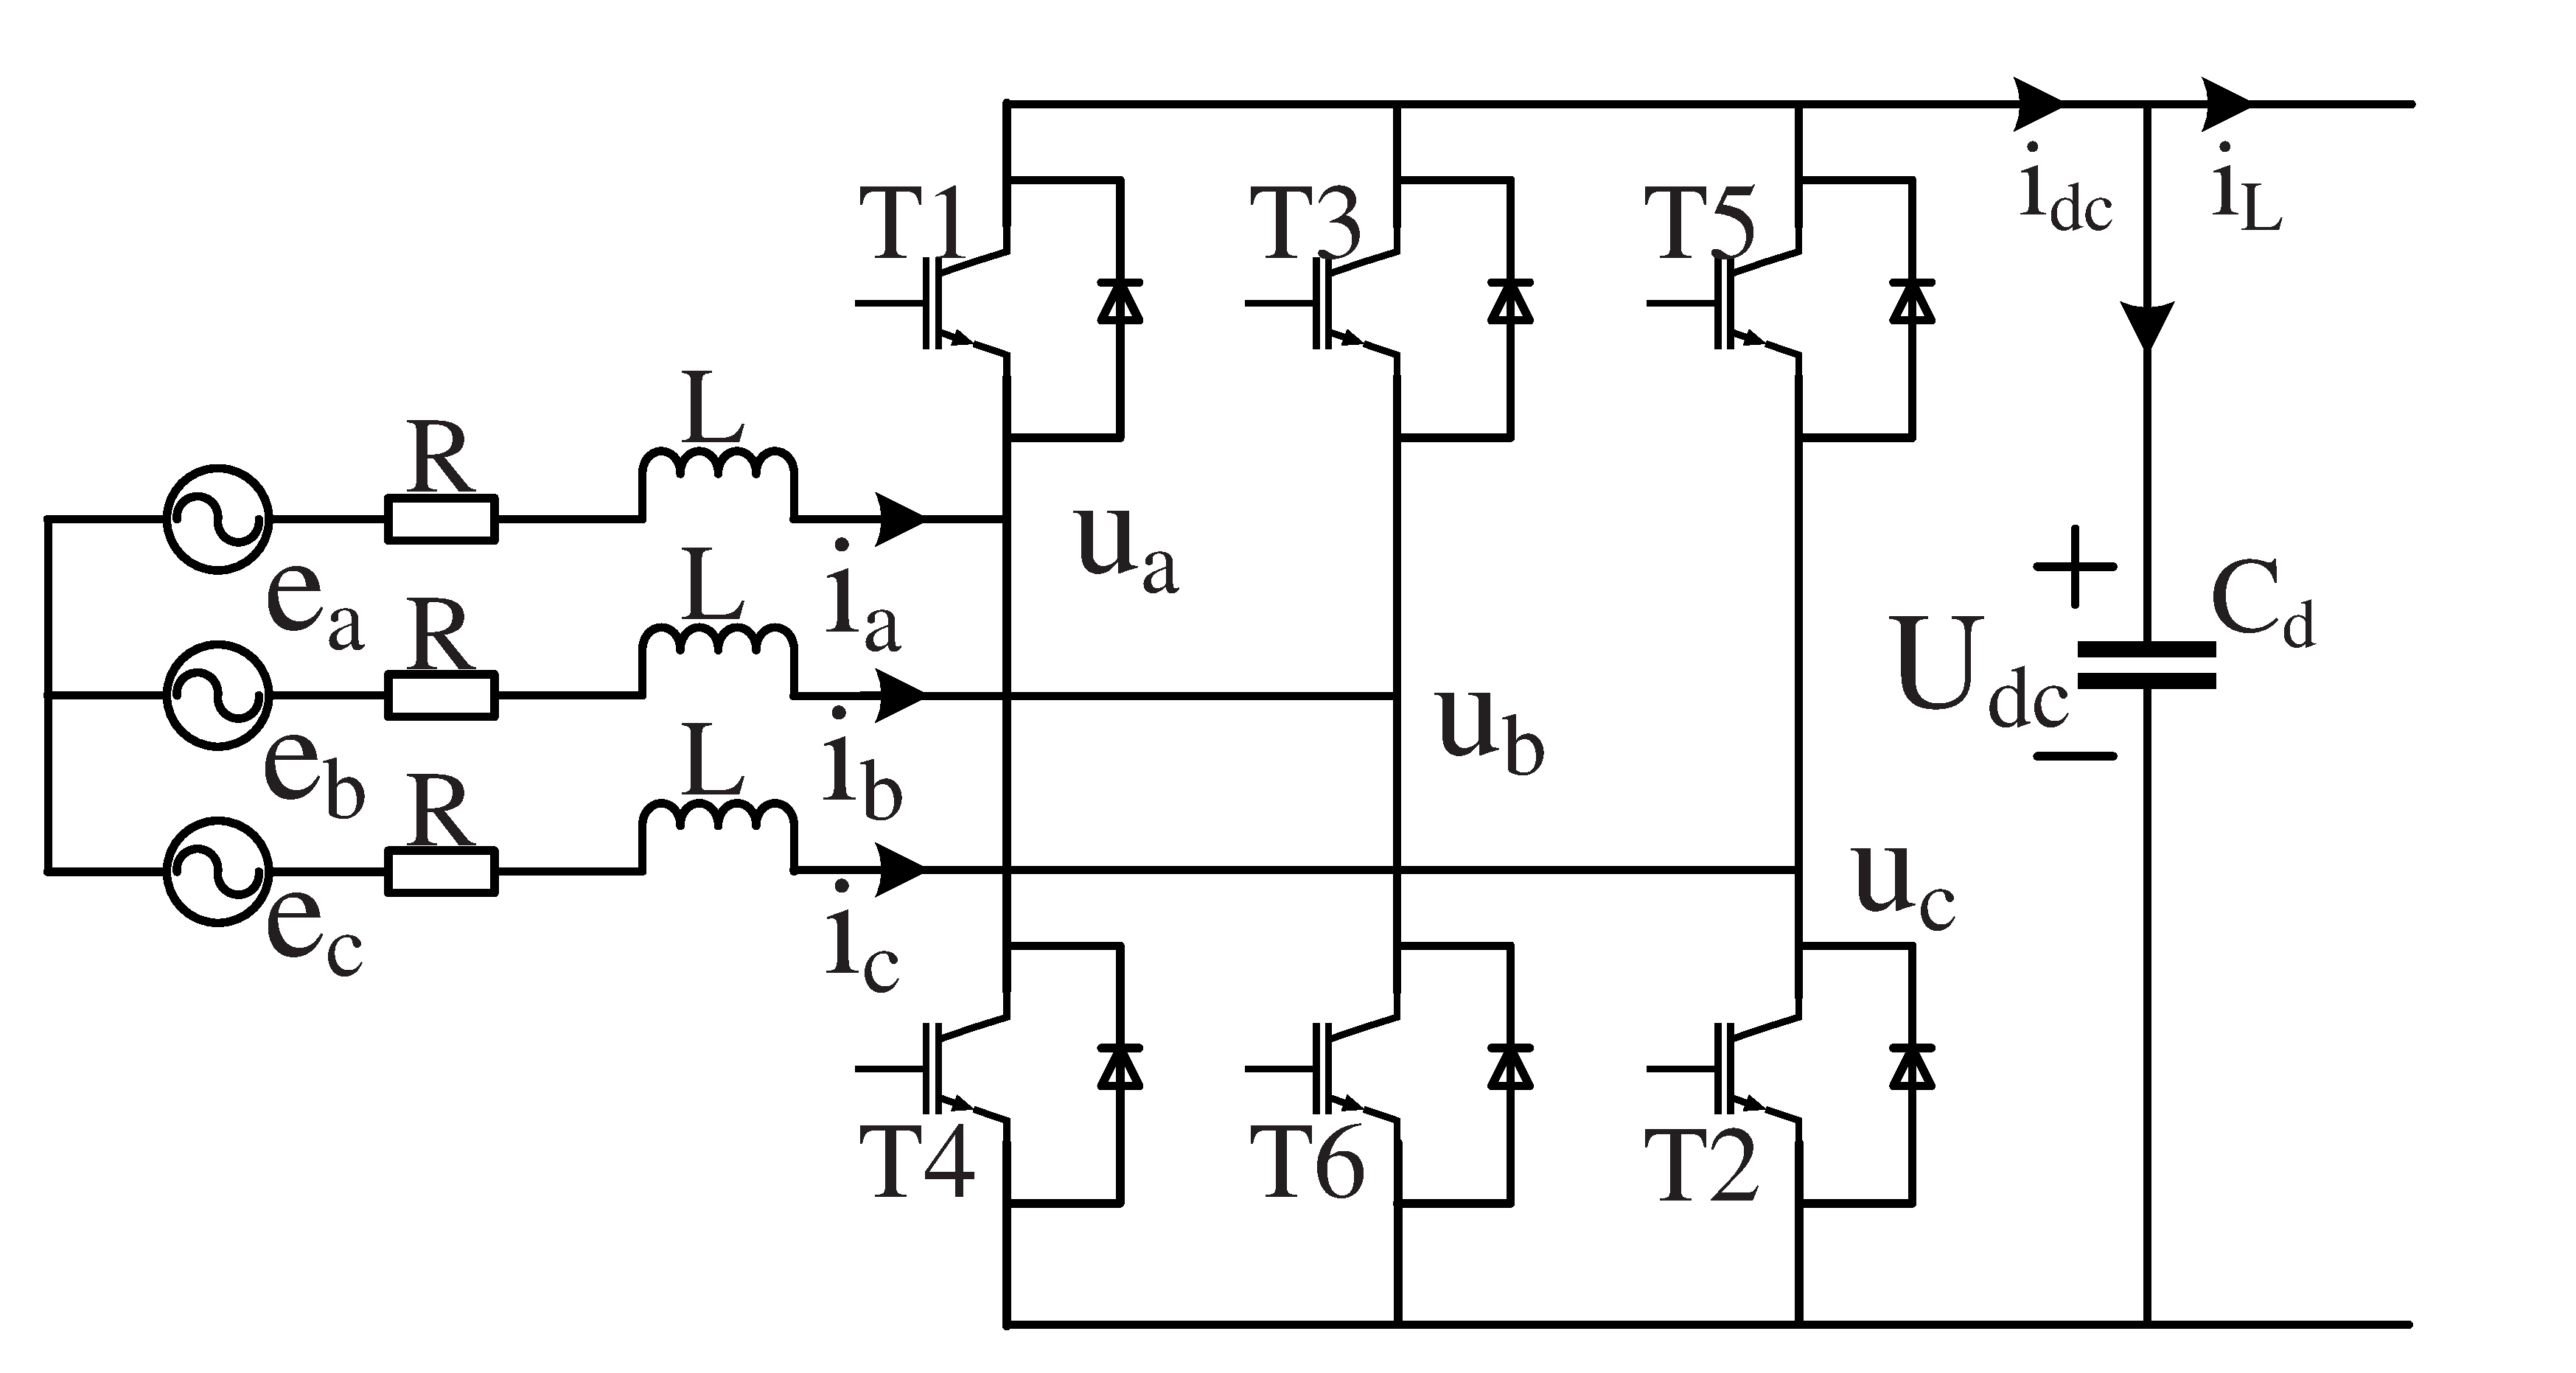
\includegraphics[width=0.65\textwidth]{chapter3/VSR/VSR拓扑.pdf}
	\caption{三相VSR拓扑结构图}
	\label{fig:三相VSR拓扑结构图}
\end{figure}

\begin{equation}
	s_{k} =
	\begin{cases}
		1 \quad \text{上桥臂IGBT导通,下桥臂IGBT关断} \\
		0 \quad \text{上桥臂IGBT关断,下桥臂IGBT导通} \\
	\end{cases}
	(k=a,b,c)
	\label{equ:Sk}
\end{equation}

\begin{equation}
	L\frac{di_{u}}{dt}+Ri_{u}=e_{u}-(u_{uN}+u_{NO})
	\label{equ:3-3}
\end{equation}

\begin{equation}
	L\frac{di_{u}}{dt}+Ri_{u}=e_{u}-(u_{dc}s_{u}+u_{NO})
\end{equation}
同样的v,w相
\begin{equation}
	L\frac{di_{v}}{dt}+Ri_{v}=e_{v}-(u_{dc}s_{v}+u_{NO})
	\label{equ:3-4}
\end{equation}

\begin{equation}
	L\frac{di_{w}}{dt}+Ri_{w}=e_{w}-(u_{dc}s_{w}+u_{NO})
	\label{equ:3-5}
\end{equation}
三相对称,所以有:
\begin{equation}
	e_{u}+e_{v}+e_{w}=0
	\label{equ:3-6}
\end{equation}

\begin{equation}
	i_{u}+i_{v}+i_{w}=0 
	\label{equ:3-7}
\end{equation}
将式(\ref{equ:3-6})式(\ref{equ:3-7})代入式(\ref{equ:3-3})~\~{}式(\ref{equ:3-5})中得:
\begin{equation}
	u_{NO}=-\frac{u_{dc}}{3} \left ( s_{u}+s_{v}+s_{w}  \right )
\end{equation}
直流侧电流$i_{dc}$可以表示为:
\begin{equation}
	i_{dc}=i_{u}s_{u}+i_{v}s_{w}+i_{w}s_{w}
\end{equation}
直流侧电容电流:
\begin{equation}
	C\frac{du_{dc}}{dt}=i_{u}s_{u}+i_{v}s_{w}+i_{w}s_{w}-i_{L}
\end{equation}

设状态变量$\boldsymbol{X}=[i_{u},i_{v},i_{w},u_{dc}]^{T}$,
输入变量$\boldsymbol{U}=[e_{u},e_{v},e_{w},i_{L}]^{T}$则三项VSR状态空间可以表示为:

\begin{equation}
	\boldsymbol{\dot{X}}=\boldsymbol{AX}+\boldsymbol{BU}
\end{equation}
上式中:
\begin{equation}
	\boldsymbol{A}=
	\begin{pmatrix}
		-\frac{R}{L}    & 0               & 0               & -\frac{1}{L}  ( s_{u}-\frac{1}{3} \sum\limits_{k=u,v,w} s_{k}  ) \\
		0               & -\frac{R}{L}    & 0               & -\frac{1}{L}  ( s_{u}-\frac{1}{3} \sum\limits_{k=u,v,w} s_{k}  ) \\
		0               & 0               & -\frac{R}{L}    & -\frac{1}{L}  ( s_{u}-\frac{1}{3} \sum\limits_{k=u,v,w} s_{k}  ) \\
		\frac{s_{a}}{C} & \frac{s_{b}}{C} & \frac{s_{c}}{C} & 0
	\end{pmatrix}
\end{equation}

\begin{equation}
	\boldsymbol{B}=
	\begin{pmatrix}
		\frac{1}{L} & 0           & 0           & 0            \\
		0           & \frac{1}{L} & 0           & 0            \\
		0           & 0           & \frac{1}{L} & 0            \\
		0           & 0           & 0           & -\frac{1}{C}
	\end{pmatrix}
\end{equation}
三相VSR的数学模型结构如图\ref{fig:三相VSR一般数学模型结构}所示:

\begin{figure}[!htp]
	\centering
	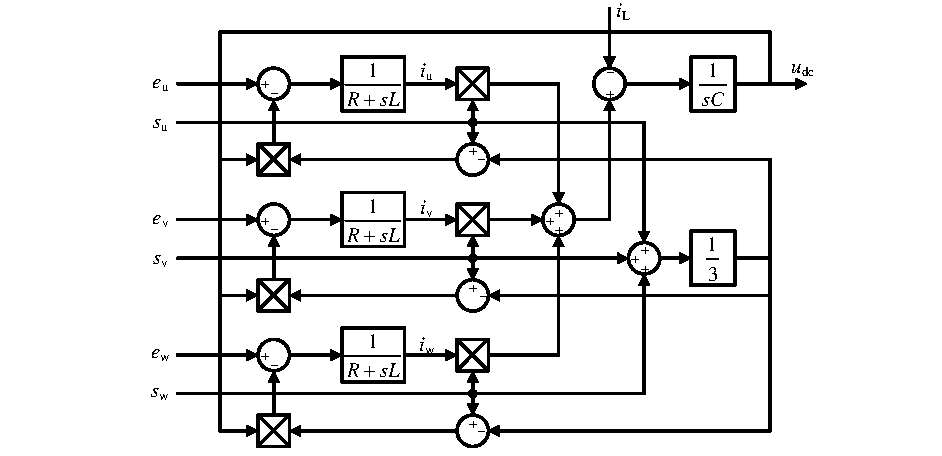
\includegraphics[width=0.9\textwidth]{chapter3/VSR/三相VSR一般数学模型结构.pdf}
	\caption{三相VSR一般数学模型结构}
	\label{fig:三相VSR一般数学模型结构}
\end{figure}

前文对三相静止abc坐标系中的VSR一般数学模型进行了分析,此模型具有物理意义清晰、直观等特点。
但在一般数学模型中,VSR网侧均为时变交流量,不利于控制系统设计。鉴于此,可以通过坐标变换将三相静止abc
坐标系转换成以网侧电动势基波角频率同步旋转的dq坐标系。坐标变换后,三相交变量转化成同步旋转坐标系中的直流量,
从而简化了控制系统的设计。

为将三相静止abc坐标系转换成同步旋转dq坐标系,首先可将三相静止坐标系转换成两相静止$\alpha\beta$坐标系。
设有通用矢量$\boldsymbol{X}$ ,
其在$\alpha$、$\beta$轴上的投影为$x_{\alpha}$、$x_{\beta}$,在a、b、c轴上的投影为$x_{a}$、$x_{b}$、$x_{c}$,
令a轴与α轴重合,则有:

\begin{equation}
	\begin{pmatrix}
		x_{\alpha } \\
		x_{\beta }
	\end{pmatrix}
	=
	\frac{2}{3}
	\begin{pmatrix}
		1 & -\frac{1}{2}         & -\frac{1}{2}        \\
		0 & -\frac{\sqrt{3} }{2} & \frac{\sqrt{3} }{2}
	\end{pmatrix}
	\begin{pmatrix}
		x_{a} \\
		x_{b} \\
		x_{c}
	\end{pmatrix}
	\label{equ:abc2αβ}
\end{equation}
或
\begin{equation}
	\begin{pmatrix}
		x_{a} \\
		x_{b} \\
		x_{c}
	\end{pmatrix}
	=
	\begin{pmatrix}
		1            & 0                    \\
		-\frac{1}{2} & -\frac{\sqrt{3} }{2} \\
		-\frac{1}{2} & \frac{\sqrt{3} }{2}
	\end{pmatrix}
	\begin{pmatrix}
		x_{\alpha } \\
		x_{\beta }
	\end{pmatrix}
\end{equation}
对于三相VSR有:
\begin{equation}
	\begin{cases}
		x_{k}\in  \{ e_{k},e_{k},s_{k} \} \quad(k=a,b,c)          \\
		x_{l}\in  \{ e_{l},e_{l},s_{l} \} \quad(l=\alpha ,\beta ) \\
		x_{j}\in  \{ e_{j},e_{j},s_{j} \} \quad(j=d,q)
	\end{cases}
\end{equation}
化简,可得两相静止坐标系中三相 VSR 开关函数模型为:
\begin{equation}
	\begin{cases}
		C \frac{\mathrm{d} u_{\mathrm{dc}}}{\mathrm{d} t}=\frac{3}{2}\left(i_{\alpha} s_{\alpha}+i_{\beta} s_{\beta}\right)-i_{\mathrm{L}} \\
		L \frac{\mathrm{d} i_{\alpha}}{\mathrm{d} t}+R i_{\alpha}=e_{\alpha}-u_{\mathrm{dc}} s_{\alpha}                                    \\
		L \frac{\mathrm{d} i_{\beta}}{\mathrm{d} t}+R i_{\beta}=e_{\beta}-u_{\mathrm{dc}} s_{\beta}
	\end{cases}
	\label{equ:3-17}
\end{equation}
两相静止坐标系到同步旋转坐标系的转换矩阵为:
\begin{equation}
	\begin{pmatrix}
		x_{\alpha } \\
		x_{\beta }
	\end{pmatrix}=
	\begin{pmatrix}
		cos\varphi & -sin\varphi \\
		sin\varphi & cos\varphi
	\end{pmatrix}
	\begin{pmatrix}
		x_{d } \\
		x_{q}
	\end{pmatrix}
	\label{equ:αβ2dq变换公式}
\end{equation}
式中,$\varphi$为d轴与$\alpha$轴的夹角。将式(\ref{equ:αβ2dq变换公式})代入式(\ref{equ:3-17}),得到
三相VSR在dq坐标系下的数学模型:
\begin{equation}
	\begin{cases}
		C \frac{\mathrm{d} u_{\mathrm{dc}}}{\mathrm{d} t}=\frac{3}{2}\left(i_{\mathrm{d}} s_{\mathrm{d}}+i_{\mathrm{q}} s_{\mathrm{q}}\right)-i_{\mathrm{L}} \\
		L \frac{\mathrm{d} i_{\mathrm{d}}}{\mathrm{d} t}+R i_{\mathrm{d}}-\omega L i_{\mathrm{q}}=e_{\mathrm{d}}-u_{\mathrm{dc}} s_{\mathrm{d}}              \\
		L \frac{\mathrm{d} i_{\mathrm{q}}}{\mathrm{d} t}+R i_{\mathrm{q}}+\omega L i_{\mathrm{d}}=e_{\mathrm{q}}-u_{\mathrm{dc}} s_{\mathrm{q}}
	\end{cases}
	\label{equ:VSR dq数学模型}
\end{equation}

\begin{figure}[!htp]
	\centering
	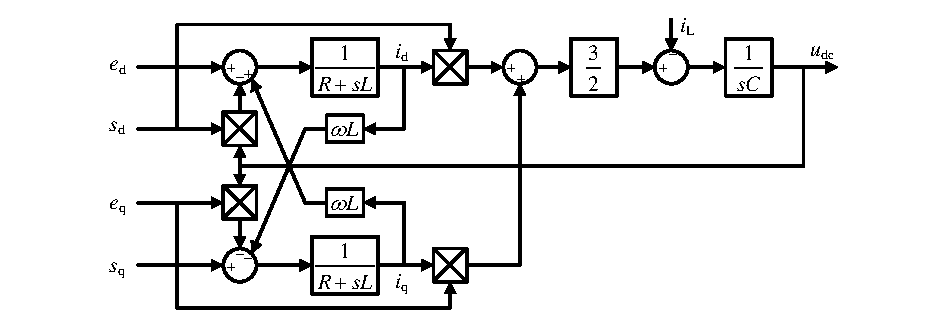
\includegraphics[width=\textwidth]{chapter3/VSR/三相VSR dq数学模型结构.pdf}
	\caption{三相VSR dq数学模型结构.pdf}
	\label{fig:三相VSR dq数学模型结构.pdf}
\end{figure}

\subsection{变流器逆变侧模型}

\begin{figure}[!htp]
	\centering
	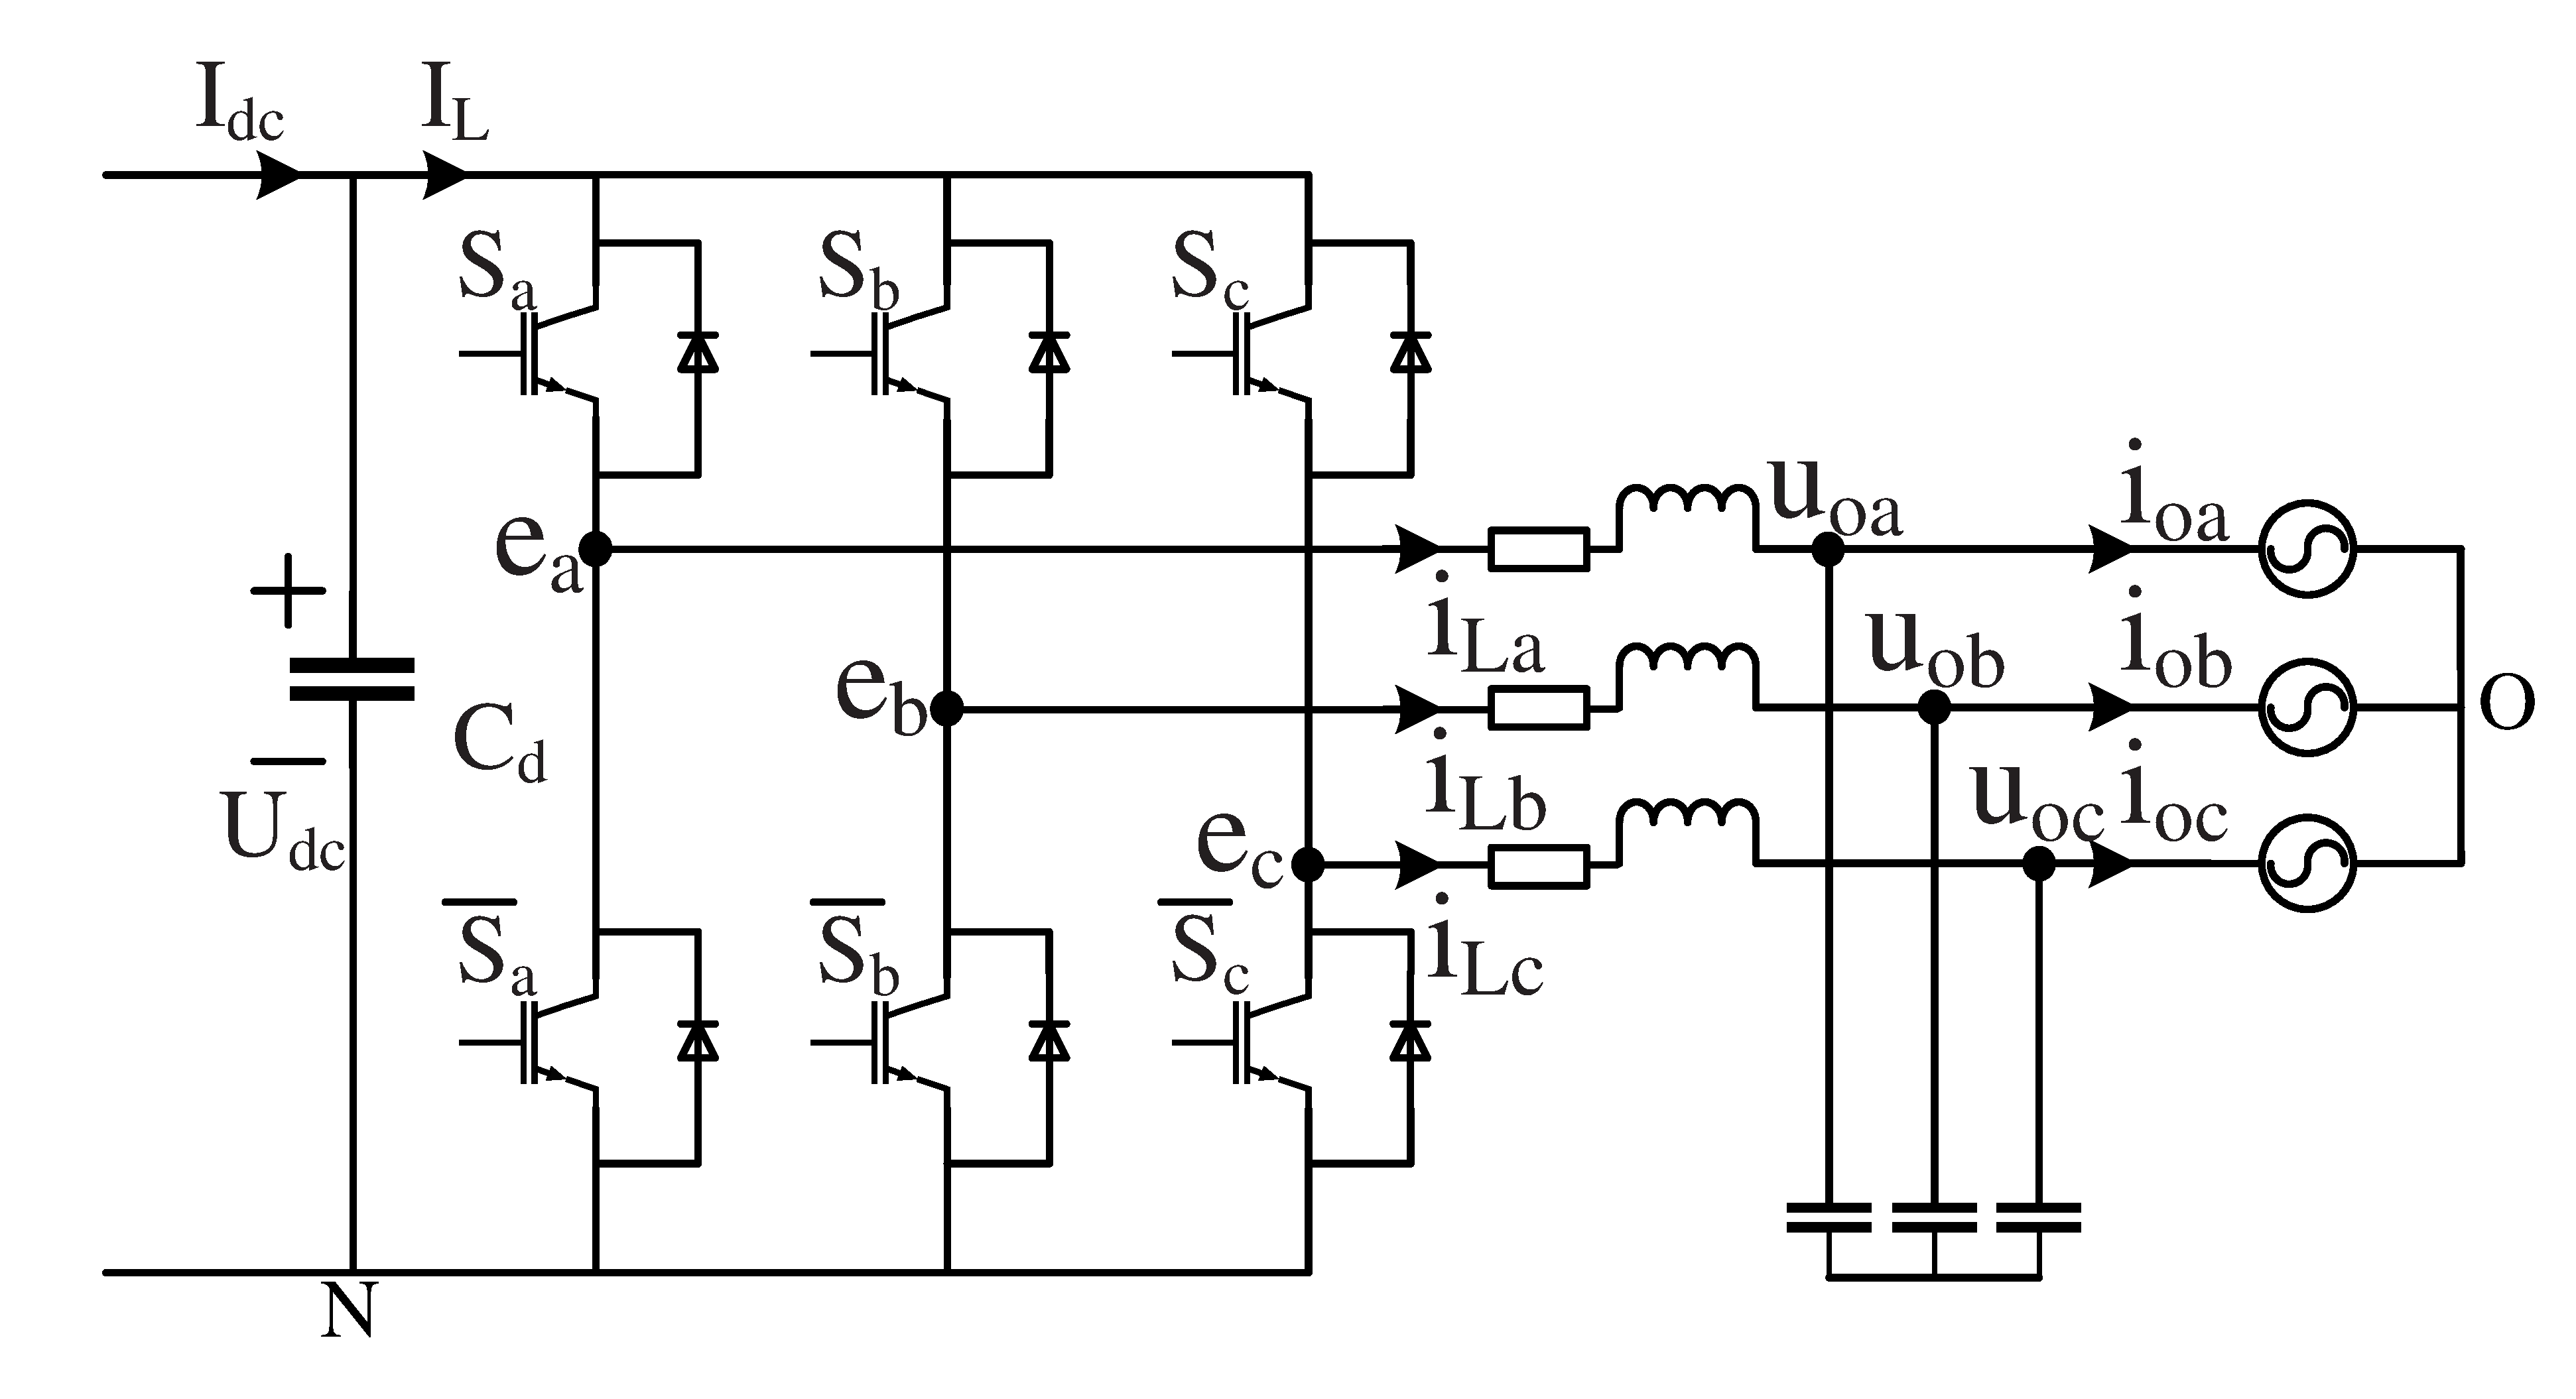
\includegraphics[width=0.65\textwidth]{chapter3/VSI/VSI拓扑.pdf}
	\caption{三相VSI拓扑结构图}
	\label{fig:三相VSI拓扑结构图}
\end{figure}
同三相 VSR 一样,首先定义单极性二值逻辑开关函数$s_{k}$为:
\begin{equation}
	s_{j} =
	\begin{cases}
		1 \quad \text{上桥臂IGBT导通,下桥臂IGBT关断} \\
		0 \quad \text{上桥臂IGBT关断,下桥臂IGBT导通} \\
	\end{cases}
	(j=a,b,c)
	\label{equ:Sk}
\end{equation}
根据基尔霍夫电压定律建立三相VSI回路方程:
\begin{equation}
	\begin{cases}
		L \frac{d i_{La}}{dt}+R i_{La}=e_{a}-u_{oa}-u_{ON} \\
		L \frac{d i_{Lb}}{dt}+R i_{Lb}=e_{b}-u_{ob}-u_{ON} \\
		L \frac{d i_{Lc}}{dt}+R i_{Lc}=e_{c}-u_{oc}-u_{ON}
	\end{cases}
	\label{equ:3-21}
\end{equation}
将$e_{k}=u_{dc}s_{k}\quad(k=a,b,c)$代入式(\ref{equ:3-21})得:
\begin{equation}
	\begin{cases}
		L\frac{di_{La}}{dt}+Ri_{La}=u_{dc}s_{a}-u_{oa}-u_{ON} \\
		L\frac{di_{Lb}}{dt}+Ri_{Lb}=u_{dc}s_{b}-u_{ob}-u_{ON} \\
		L\frac{di_{Lc}}{dt}+Ri_{Lc}=u_{dc}s_{c}-u_{oc}-u_{ON}
		\label{equ:VSI model1}
	\end{cases}
\end{equation}
考虑到三相对称性,则有:
\begin{equation}
	i_{La}+i_{Lb}+i_{Lc}=0 \quad u_{oa}+u_{ob}+u_{oc}=0 \label{equ:3-23}
\end{equation}
联立式(\ref{equ:VSI model1})和式(\ref{equ:3-23})得:
\begin{equation}
	u_{ON}=\frac{u_{dc}}{3}\sum_{k=a,b,c}s_{k}
\end{equation}
根据基尔霍夫电流定律建立整流侧电容电流方程和滤波电容节点处电流方程:
\begin{equation}
	\begin{cases}
		C\frac{du_{oa}}{dt}=i_{La}-i_{oa} \\
		C\frac{du_{ob}}{dt}=i_{Lb}-i_{ob} \\
		C\frac{du_{oc}}{dt}=i_{Lc}-i_{oc} \\
		C\frac{du_{dc}}{dt}=i_{dc}-i_{L}
	\end{cases}
\end{equation}

设状态变量$\boldsymbol{X}=[i_{La},i_{Lb},i_{Lc},u_{dc}]^{T}$,
输入变量$\boldsymbol{U}=[e_{oa},e_{ob},e_{oc},i_{L}]^{T}$则三项VSR状态方程可以表示为:
\begin{equation}
	\boldsymbol{\dot{X}}=\boldsymbol{A}\boldsymbol{X}+\boldsymbol{B}\boldsymbol{E}+\boldsymbol{Z}
\end{equation}
上式中:
\begin{equation}
	\boldsymbol{A}=
	\begin{pmatrix}
		-\frac{R}{L}    & 0               & 0               & - \frac{1}{3L} \sum\limits_{k=u,v,w} s_{k} \\
		0               & -\frac{R}{L}    & 0               & - \frac{1}{3L} \sum\limits_{k=u,v,w} s_{k} \\
		0               & 0               & -\frac{R}{L}    & - \frac{1}{3L} \sum\limits_{k=u,v,w} s_{k} \\
		\frac{s_{a}}{C} & \frac{s_{b}}{C} & \frac{s_{c}}{C} & 0
	\end{pmatrix}
\end{equation}

\begin{equation}
	\boldsymbol{B}=
	\begin{pmatrix}
		-\frac{1}{L} & 0            & 0            & 0            \\
		0            & -\frac{1}{L} & 0            & 0            \\
		0            & 0            & -\frac{1}{L} & 0            \\
		0            & 0            & 0            & -\frac{1}{C}
	\end{pmatrix}
\end{equation}

\begin{equation}
	\boldsymbol{Z}=
	\begin{pmatrix}
		0 & 0 & 0 & \frac{i_{dc}}{C}
	\end{pmatrix}^{T}
\end{equation}

与整流侧类似,为了得到三相VSI dq数学模型,新疆abc静止坐标系转换为两相静止$\alpha\beta$坐标系。
结合式(\ref{equ:abc2αβ})与式(\ref{equ:VSI model1})得到三相VSI$\alpha\beta$模型:
\begin{equation}
	\begin{cases}
		L\frac{di_{L\alpha}}{dt}=-Ri_{L\alpha}+e_{\alpha}-u_{o\alpha} \\
		L\frac{di_{L\beta}}{dt}=-Ri_{L\beta}+e_{\beta}-u_{o\beta}
	\end{cases}
	\label{equ:VSI αβ model1}
\end{equation}

\begin{equation}
	\begin{cases}
		C\frac{du_{o\alpha}}{dt}=i_{L\alpha}-i_{o\alpha} \\
		C\frac{du_{o\beta}}{dt}=i_{L\beta}-i_{o\beta}
	\end{cases}
	\label{equ:VSI αβ model2}
\end{equation}

为使两相静止$\alpha\beta$坐标系转化为同步旋转dq坐标系,将式(\ref{equ:αβ2dq变换公式})代入
式(\ref{equ:VSI αβ model1})和式(\ref{equ:VSI αβ model2})中,整理得到VSI dq模型:
\begin{equation}
	\begin{cases}
		L\frac{di_{Ld}}{dt}=-Ri_{Ld}+e_{d}+\omega Li_{Lq}-u_{od} \\
		L\frac{di_{Lq}}{dt}=-Ri_{Lq}+e_{q}-\omega Li_{Ld}-u_{oq}
	\end{cases}
	\label{equ:VSI dq model1}
\end{equation}

\begin{equation}
	\begin{cases}
		C\frac{du_{od}}{dt}=i_{Ld}+\omega Cu_{oq}-i_{od} \\
		C\frac{du_{oq}}{dt}=i_{Ld}-\omega Cu_{oa}-i_{oq}
	\end{cases}
	\label{equ:VSI dq model2}
\end{equation}

三相VSI dq模型结构,如图\ref{fig:两相同步旋转dq坐标系中三相VSI模型结构图}所示。

\begin{figure}[!htp]
	\centering
	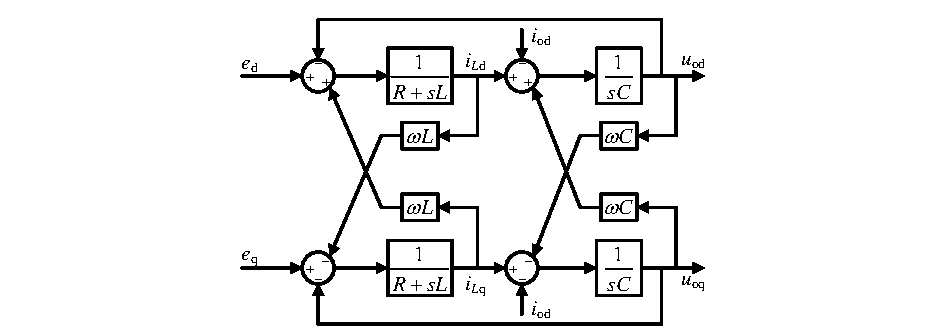
\includegraphics[width=\textwidth]{chapter3/VSI/两相同步旋转坐标系中三相VSI模型结构图.pdf}
	\caption{两相同步旋转dq坐标系中三相VSI模型结构图}
	\label{fig:两相同步旋转dq坐标系中三相VSI模型结构图}
\end{figure}


\subsection{岸侧变压器模型}




\subsection{岸侧滤波器模型}


\section{岸侧变流器系统控制策略}

电压电流瞬时值双闭环控制的系统框图,它的原理为:采样岸电电源的输出电压U0,经过信号调理获得电压反馈信号Vfed,
并和电压给定值Vref相比较得到偏差信号ev。然后送入电压调节器,它的输出值即是电流内环反馈的参考
值Iref,再和电流反馈值If相比较获得误差信号ei。最后经过电流调节器得到控制信号Vc并输出给DSP进行运算处理,
从而对SPWM驱动波形进行调制。

\begin{figure}[!htp]
	\centering
	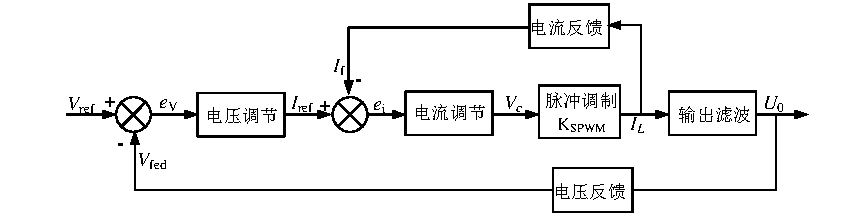
\includegraphics[width=\textwidth]{chapter3/电压电流双闭环控制.pdf}
	\caption{压电流双闭环控制}
	\label{fig:压电流双闭环控制}
\end{figure}

\subsection{变流器整流侧控制方法}

电流内环,电压外环双闭环控制策略。

\begin{figure}[!htp]
	\centering
	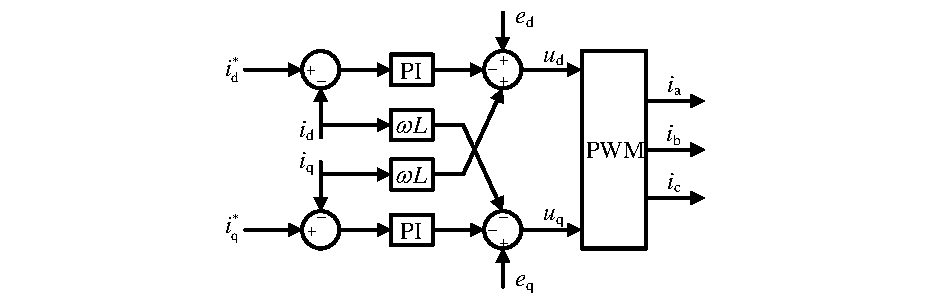
\includegraphics[width=0.9\textwidth]{chapter3/VSR/三相VSR电流内环解耦控制结构.pdf}
	\caption{三相VSR电流内环解耦控制结构}
	\label{fig:三相VSR电流内环解耦控制结构}
\end{figure}

\begin{figure}[!htp]
	\centering
	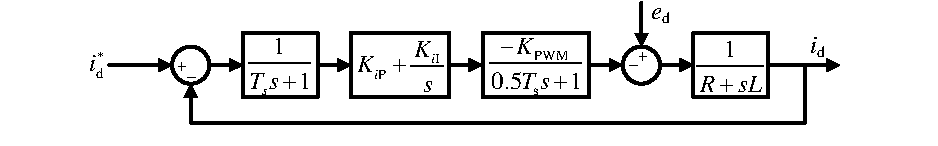
\includegraphics[width=\textwidth]{chapter3/VSR/id电流内环结构.pdf}
	\caption{id电流内环结构}
	\label{fig:id电流内环结构}
\end{figure}

\begin{figure}[!htp]
	\centering
	
\includegraphics[width=\textwidth]{chapter3/VSR/无ed扰动时的id电流内环结构.pdf}
	\caption{无ed扰动时的id电流内环结构.pdf}
	\label{fig:无ed扰动时的id电流内环结构.pdf}
\end{figure}

\begin{figure}[!htp]
	\centering
	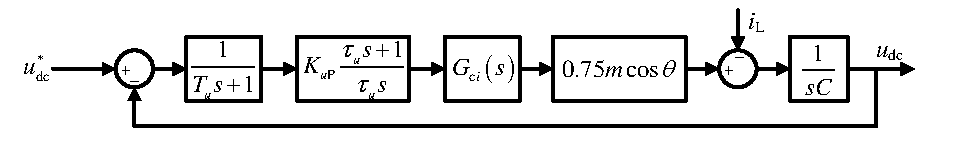
\includegraphics[width=\textwidth]{chapter3/VSR/三相VSR电压外环控制结构.pdf}
	\caption{三相VSR电压外环控制结构}
	\label{fig:三相VSR电压外环控制结构}
\end{figure}

\begin{figure}[!htp]
	\centering
	
\includegraphics[width=\textwidth]{chapter3/VSR/三相VSR电压外环简化结构.pdf}
	\caption{三相VSR电压外环简化结构}
	\label{fig:三相VSR电压外环简化结构}
\end{figure}

\subsection{变流器逆变侧控制方法}

电流内环,电压外环双闭环控制策略。

\begin{figure}[!htp]
	\centering
	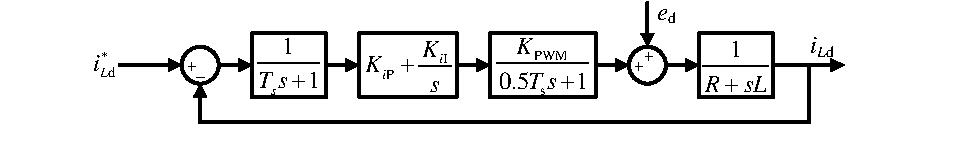
\includegraphics[width=\textwidth]{chapter3/VSI/iLd电流内环结构.pdf}
	\caption{iLd电流内环结构}
	\label{fig:iLd电流内环结构}
\end{figure}

\begin{figure}[!htp]
	\centering
	
\includegraphics[width=\textwidth]{chapter3/VSI/无ed扰动时的iLd电流内环结构.pdf}
	\caption{无ed扰动时的iLd电流内环结构}
	\label{fig:无ed扰动时的iLd电流内环结构}
\end{figure}

\begin{figure}[!htp]
	\centering
	
\includegraphics[width=\textwidth]{chapter3/VSI/Uod电压外环结构.pdf}
	\caption{Uod电压外环结构}
	\label{fig:Uod电压外环结构}
\end{figure}

\begin{figure}[!htp]
	\centering
	
\includegraphics[width=\textwidth]{chapter3/VSI/Uod电压外环简化结构.pdf}
	\caption{Uod电压外环简化结构}
	\label{fig:Uod电压外环简化结构}
\end{figure}

\section{岸电电力系统仿真}

搭建如图\ref{fig:低压岸电系统仿真示意图}所示的岸电仿真模型。

\begin{figure}[!htp]
	\centering
	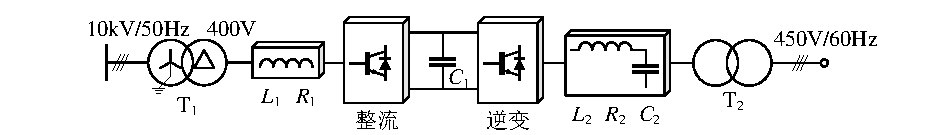
\includegraphics[width=\textwidth]{chapter3/低压岸电换流系统仿真结构示意图.pdf}
	\caption{一种低压岸电系统仿真示意图}
	\label{fig:低压岸电系统仿真示意图}
\end{figure}

\section{船舶电力系统模型与分析}

\subsection{船舶柴油发电机调速模型}

\subsection{同步发电机模型}

\subsection{发电机励磁系统模型}

\subsection{船舶负载模型}

\section{船舶电力系统仿真}



\section{系统压降解决方案}

岸基电源输出至接线箱的压降主要有两部分: 输出隔离变压器、输出电缆。

\subsection{隔离变压器的压降问题}

在不同的负载下,隔离变压器压降不同,负载越重,压降越大,针对这一部分问题,解决方案有两种:

方案一: 变频电源对隔离变压器输出侧电压进行采集,将信号传输至变频主控系统,由主控系统进行闭环控制,
稳定控制隔离变压器输出侧电压稳定,此方案控制相对更加精准。

方案二: 根据隔离变压器的阻抗值,将阻抗值输入变频主控算法中,由变频对此压降进行补偿,此方案相对简单。

\subsection{输出电缆的压降问题}

根据不同长度的输出电缆,其压降不同,但总体压降不多,针对此部分压降,可采用电压微调的方式进行,电压微调可通过触摸屏修改。


\section{船舶岸电供电并网切换}
船岸电力的电网连接是在船的柴油发电机和岸上电源之间。并网需要满足四个条件:船舶发电机的相序、幅值、相位、频率
必须与岸电一致。保持相同的相序尤为重要。影响瞬时电压差的三个因素是频率差、相位差和电压差。船岸自动准同步并网
的四个条件如下:
(1)船舶电源的相序必须等于岸上电源的相序;
(2)船舶电源的电压幅值必须等于岸上电源的电压幅值;
(3)船舶电源的频率必须等于岸上电源的频率;
(4)船舶电源的相位必须等于岸上电源的相位。
这些条件在理想情况下得到满足。事实上,相位、频率和振幅不可能同时完全一致。但只要船电和岸电的相位、频率、幅度差
在一定值内,涌流就在系统可接受的范围内,所以可以进行船岸并网。

船舶岸电系统具备船电、岸电快速切换连接技术,通过船上同期装置,与岸电电源实现热并网,保证供电安全
可靠。船舶 岸电 系统接到岸电并网指令后,自动并车装置进行相序检测跟踪,在相序一致的情况 下,采集岸电电源及传
播辅机电源的电压、频率和相角差的信息,并计算判断是否满足以下并车条件:辅机与岸电的频率、相序及 电压幅值保持
一致,并且在并车的瞬间保证船舶辅机与岸电电源的输出电压相角同步。之后 完成并车并实现自动无缝负荷转移。根据船舶岸电
系统不同的供电连接方式,将岸电电源与船舶发电机的切换方式主要分为断电方式和无缝切换方式2种\cite{SP10}。
1)断电方式:当船舶靠港停泊时,需要首先使船舶上所有的用电设备关闭,并使船舶发电机停止工作,然后连接船舶岸电
系统,最后重新启动船舶的用电设备,实现船舶发电机与岸电电源之间的切换;当船舶离港时,按照相反的顺序操作。
2)同步并车方式:也被称为无缝切换方式,切换过程中不需要关闭 船上所有设备。同步并车方式不会影响船舶上用电设备
的正常运行,对船舶上的重要用电设备具有重大意义。无缝切换也是船舶岸电连接技术的发展趋势,对于岸电电源的推广
意义重大。船舶岸电自动并车技术需要保证船舶发电机与岸电电源的电压幅值和频率保持一致,并在并车的瞬间保证船舶发
电机与岸电电 源的输出电压相角同步。如果两路电源不同步就进行切换会造成严重的后果。如果在切换时刻一个电源电压波
形在波峰,另外一个位于波谷,切换过程中将会产生很大的冲击电流。虽然切换装置可能能承受该冲击电流,但严重时可能
会导致用电设备和高压静止频率变换器的自动保护装置动作。

岸电与船舶辅机并网,船舶保证不停电,实现无缝切换方式,变频电源具有主动切换与被动切换两种方式,具体实现如下:

\subsection{主动并网切换}

变频电源仅作为整个电网切换的主体变频,根据采集到的船上辅机发电机发出电源的信息,包括电压及电流。电压信号主要
用于变频输出电压的标准,变频输出锁频锁相,使输出电源的相位、频率、幅值、相序等与船上完全一致。

电流信息主要作用是让变频控制器获得此时发电机的输出功率,进行负载转移,变频控制器可控制输出,使输出功率逐渐增
大,直至将发电机所带负载完全转移至变频电源供电。

主动切换方式目前有少部分应用,其优点是可以做到整个切换过程的智能化,如一键切换,中间所有过程可自动全部完成。
缺点是需要船方的配合进行改造,否则无法知道发电机的电压、电流等信息,系统不具通用性。

\subsection{被动并网切换}

变频电源仅作为恒频稳压的电源,按照要求输出电压及频率,所有的电网之间的切换均依靠船上的同期柜,具体步骤如下:

变频根据命令要求输出电压 /频率,电源通过输出滤波、隔离变、接口箱、船上进线柜,直接送至船载的变频电源并网柜,
并网柜根据采集到的信息,显示电源的相序、频率、幅值、相位等信息,自动判断是否具备并网条件,通过调整发电机的发
电信息,直至具备并网条件后将变频电源接入; 成功并网后,发电机减小输出功率,负载自动逐渐转移至岸用电源供电,切
换完成后,发电机退出工作。

被动切换是目前比较流行、采用最多的方案,因为其具有简单、通用等特点,且可以实现单个电源同时给多条船只供电的情
况; 但缺点是目前船上与岸基电源之间除了安全联锁信号外,没有其他信号交互,自动化程度低,主要原因是岸电电源与船
上之间的通信协议还未形成国际标准。

\section{逆功率处理方案}

\subsection{逆功率产生机理}

岸用电源逆功率产生的机理如图所示。

两个电压源同时给负载供电时,由于并网运行时的相位、频率和幅值之差导致的逆功率。下面从矢量图分析几种逆功率产生
的机理,V1 为岸用电源,V2 为发电机电源。

V→1超前V→2,V→1与i→s夹角θ小于90°,不会出现逆功率情况,如图所示。

\subsection{逆功率的处理}

(1) 检测到逆功率状态时,变频电源主动调节输出频率及输出相位,使V→1与i→s夹角小于 90°,通过软件算法从根本
上解决逆功率问题,主动抑制逆功率的产生;

(2) 采用四象限变频器,当产生逆功时,通过回馈到电网的方式来解决;

(3) 制动电阻吸收方式,当产生逆功时,通过制动电阻来吸收产生的能量。

\subsection{不同控制方案简单对比}

由于逆功率控制仅用于并网瞬间即解列过程,整个过程大概几秒时间,不同的控制方案达到的实际效果不同,
具体对比如表所示。

\section{并网负载转移}

不同船舶的主配电板不一样,并网的切换方式也不一样。日本峙崎和日本 JRCS 的船舶主配电板,并网负载转移方式是按
照负载容量为转移切换的依据,剩余10\% 负载时,柴油发电机退出。

长荣集团船舶、韩国现代船舶主配电板,并网负载转移方式是按照时间为转移的依据,并网后 5 s 船舶柴油发电机退出,
负载直接突加到岸电。

\section{自动电压平衡}

\section{三相输出电压平衡控制技术}

因变频电源的负载有别于变频器的电机类负载,船上单相负载的使用,导致其三相间负载分配不可能绝对的平衡,从而每相之间的压降
可能会有不同。通过三相输电压平衡控制技术,对三相输出电压实行闭环控制。

\section{船岸等电位处理方案}

岸电系统的接地系统相对要重点关注,虽然海水导电,但它存在电阻,船体( “地”) 和岸地因传导电阻造成电位差,有电位
差就会产生电流,威胁人身安全,故无论是低压还是岸电,均要求船岸的“地”保持等电位连接,以降低接触电压,提高安全
用电水平。在岸电连船过程中应注意该等电位连接不应改变船舶配电系统的接地原理。对于船岸之间的等电位连接设计如下:
船岸连接等电位线集成于船岸连接动力电缆中,将船舶外壳、岸电系统外壳、码头电源插座箱箱体与码头电网相连,
如图所示为等电位连接线方案。


\section{本章小结}